\documentclass[a4paper]{article}
\usepackage[]{graphicx}\usepackage[]{color}
% maxwidth is the original width if it is less than linewidth
% otherwise use linewidth (to make sure the graphics do not exceed the margin)
\makeatletter
\def\maxwidth{ %
  \ifdim\Gin@nat@width>\linewidth
    \linewidth
  \else
    \Gin@nat@width
  \fi
}
\makeatother

\definecolor{fgcolor}{rgb}{0.345, 0.345, 0.345}
\newcommand{\hlnum}[1]{\textcolor[rgb]{0.686,0.059,0.569}{#1}}%
\newcommand{\hlstr}[1]{\textcolor[rgb]{0.192,0.494,0.8}{#1}}%
\newcommand{\hlcom}[1]{\textcolor[rgb]{0.678,0.584,0.686}{\textit{#1}}}%
\newcommand{\hlopt}[1]{\textcolor[rgb]{0,0,0}{#1}}%
\newcommand{\hlstd}[1]{\textcolor[rgb]{0.345,0.345,0.345}{#1}}%
\newcommand{\hlkwa}[1]{\textcolor[rgb]{0.161,0.373,0.58}{\textbf{#1}}}%
\newcommand{\hlkwb}[1]{\textcolor[rgb]{0.69,0.353,0.396}{#1}}%
\newcommand{\hlkwc}[1]{\textcolor[rgb]{0.333,0.667,0.333}{#1}}%
\newcommand{\hlkwd}[1]{\textcolor[rgb]{0.737,0.353,0.396}{\textbf{#1}}}%
\let\hlipl\hlkwb

\usepackage{framed}
\makeatletter
\newenvironment{kframe}{%
 \def\at@end@of@kframe{}%
 \ifinner\ifhmode%
  \def\at@end@of@kframe{\end{minipage}}%
  \begin{minipage}{\columnwidth}%
 \fi\fi%
 \def\FrameCommand##1{\hskip\@totalleftmargin \hskip-\fboxsep
 \colorbox{shadecolor}{##1}\hskip-\fboxsep
     % There is no \\@totalrightmargin, so:
     \hskip-\linewidth \hskip-\@totalleftmargin \hskip\columnwidth}%
 \MakeFramed {\advance\hsize-\width
   \@totalleftmargin\z@ \linewidth\hsize
   \@setminipage}}%
 {\par\unskip\endMakeFramed%
 \at@end@of@kframe}
\makeatother

\definecolor{shadecolor}{rgb}{.97, .97, .97}
\definecolor{messagecolor}{rgb}{0, 0, 0}
\definecolor{warningcolor}{rgb}{1, 0, 1}
\definecolor{errorcolor}{rgb}{1, 0, 0}
\newenvironment{knitrout}{}{} % an empty environment to be redefined in TeX

\usepackage{alltt}
\newcommand{\SweaveOpts}[1]{}  % do not interfere with LaTeX
\newcommand{\SweaveInput}[1]{} % because they are not real TeX commands
\newcommand{\Sexpr}[1]{}       % will only be parsed by R



\usepackage[utf8]{inputenc}
\pagenumbering{arabic}
%\usepackage[ngerman]{babel}
\usepackage{a4wide,paralist}
\usepackage{amsmath, amssymb, xfrac, amsthm}
\usepackage{dsfont}
\usepackage[usenames,dvipsnames]{xcolor}
\usepackage{amsfonts}
\usepackage{graphicx}
\usepackage{caption}
\usepackage{subcaption}
\usepackage{framed}
\usepackage{multirow}
\usepackage{bytefield}
\usepackage{csquotes}
\usepackage[breakable, theorems, skins]{tcolorbox}
\usepackage{hyperref}
\usepackage{cancel}
\usepackage{bm}

\input{../../style/common}

\tcbset{enhanced}

%exercise numbering
\renewcommand{\theenumi}{(\alph{enumi})}
\renewcommand{\theenumii}{\roman{enumii}}
\renewcommand\labelenumi{\theenumi}

\font \sfbold=cmssbx10
\setlength{\oddsidemargin}{0cm} \setlength{\textwidth}{16cm}

\sloppy
\parindent0em
\parskip0.5em
\topmargin-2.3 cm
\textheight25cm
\textwidth17.5cm
\oddsidemargin-0.8cm
% \pagestyle{empty}

\newcommand{\kopf}[1] {
\hrule
\vspace{.15cm}
\begin{minipage}{\textwidth}
	{\sf \bf \huge Exercise Collection -- #1}
\end{minipage}
\vspace{.05cm}
\hrule
\vspace{1cm}}

\newcommand{\exlect}
  {\color{black} \hrule \section{Lecture exercises}}
  
\newcommand{\exexams}
  {\color{black} \hrule \section{Questions from past exams}}
  
\newcommand{\exinspo}
  {\color{black} \hrule \section{Ideas \& exercises from other sources}}

\newcounter{aufg}
\newenvironment{aufgabe}[1]
	{\color{black} \refstepcounter{aufg}
	\subsection{Exercise \arabic{aufg}: #1} 
	\noindent}
	{\vspace{0.5cm}}
	
\newenvironment{aufgabeexam}[3] % semester, main or retry exam, question number
	{\color{black} \refstepcounter{aufg}
	\subsection{Exercise \arabic{aufg}: #1, #2 exam, question #3}
	\noindent}
	{\vspace{1.5cm}}

\newcounter{loes}
\newenvironment{loesung}
	{\color{gray} \refstepcounter{loes}\textbf{Solution \arabic{loes}:}
	\\ \noindent}
	{\bigskip}

\setcounter{secnumdepth}{0}



\begin{document}
% !Rnw weave = knitr



\input{../../latex-math/basic-math.tex}
\input{../../latex-math/basic-ml.tex}

\kopf{Tuning \& Resampling}

\tableofcontents

% ------------------------------------------------------------------------------
% LECTURE EXERCISES
% ------------------------------------------------------------------------------

\dlz
\exlect
\lz

\aufgabe{benchmark experiment -- CART vs $k$-NN}{

\begin{enumerate}

  \item

    Suppose that we want to compare four different models:

    \begin{center}
    \begin{tabular}{c|c}
    \textbf{Model} & \textbf{Needs Tuning} \\
    \hline
    Logit Model (lm)      &  No \\
    CART  (rpart)          &  Yes \\
    k-NN (kknn)            &  Yes \\
    LDA (lda)              &  No
    \end{tabular}
    \end{center}

    To be able to compare the different models we use a 10-fold cross-validation as outer resampling strategy. Within the tuning of CART and k-NN we use a 5-fold cross-validation in combination with random search by drawing 200 hyperparameter configurations for each model. Our measure of interest is the AUC.


    \begin{enumerate}
      \item
        To conduct the final benchmark to compare the models, how many models need to be fitted in total?



      \item
        Giving the following benchmark result, which model is best? Explain your decision in one sentence.

\begin{knitrout}
\definecolor{shadecolor}{rgb}{0.969, 0.969, 0.969}\color{fgcolor}

{\centering 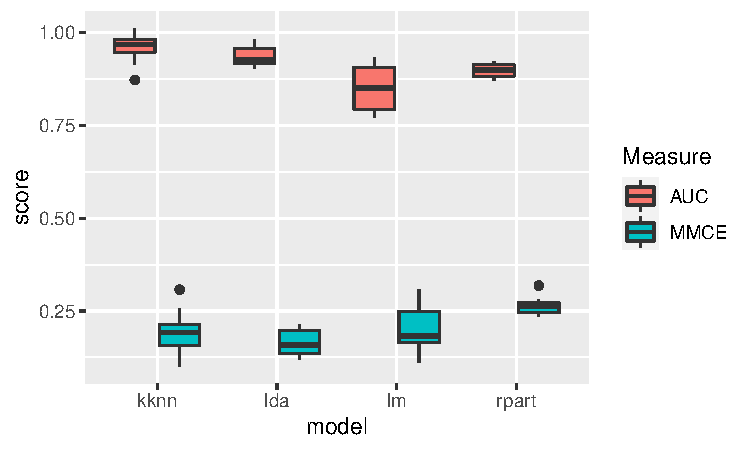
\includegraphics[width=\maxwidth]{figure/unnamed-chunk-7-1} 

}


\end{knitrout}




    \end{enumerate}

  \item
    Explain in two sentences what is meant by the \textit{bias - variance trade-off in resampling}.



  \item
    Are the following statements true or not, explain your answer in one sentence.
    \begin{enumerate}

      \item
        The bias of the generalization error for 3-fold cross-validation is higher than for 10-fold cross-validation.
   

      \item
        Every outer loss can also be used as inner loss. Assume any gradient descent based model.


    \end{enumerate}
\end{enumerate}
}

\dlz
\loesung{

\begin{enumerate}

  \item


    \begin{enumerate}
      \item



  Important parts:
  \begin{itemize}
    \item
      Correct number of models for tuning
    \item
      Correctly multiplying tuning models times the two learners that need tuning
    \item
      Correctly adding $4 \cdot 10$ for learner comparison ()
  \end{itemize}

  $$
  \# \text{models} = \underbrace{4 \cdot 10}_{\text{\# models outer resampling}} + \underbrace{2 \cdot \underbrace{10 \cdot \underbrace{5 \cdot 200}_{\text{\# models for one tuning}}}_{\text{\# models for all outer folds for one tuning}}}_{\text{\# models for both tunings}} = 20040
  $$




      \item



  We would select the k-NN (k-Nearest Neighbors) learner since it achieves the best values for the AUC.





    \end{enumerate}

  \item



  \begin{itemize}
    \item
      Less data for training leads to higher bias
    \item
      More data for training and less data for evaluation lead to higher variance
  \end{itemize}



  \item
    Are the following statements true or not, explain your answer in one sentence.
    \begin{enumerate}

      \item
          True, using 3-fold cross-validation leads to smaller train sets and therefore we are not able to learn as much as for, e.g., 10-fold cross-validation.

      \item
          False, the outer loss doesn't has as much restrictions as the inner loss, e.g. the outer loss doesn't has to be differentiable.

    \end{enumerate}
\end{enumerate}
}

\dlz
\aufgabe{benchmark study for classification}{

We want to conduct a small benchmark study:
\begin{enumerate}
\item Set up at least two datasets with a discrete target of your choice and save them in a list.
\item Set up at least three classifiers of your choice (that you are familiar with) and save them in a second list.
\item Create a resample description. Use an adequate method, depending on the size of your datasets and the complexity of the learners, so that the benchmark doesn't need hours to compute.
\item Run and visualize your benchmark study.
\end{enumerate}
}

\dlz
\loesung{

See
\href{https://github.com/compstat-lmu/lecture_i2ml/blob/master/exercises/forests/ex_rnw/sol_benchmark.R}{R code}
}

\dlz
\aufgabe{cross validation for $k$-NN}{

Use the \texttt{bodyfat} dataset from the package \texttt{TH.data} for this exercise.
\begin{enumerate}
\item Create a \texttt{mlr} regression task for the \texttt{bodyfat} data with \texttt{DEXfat} as target variable.


\item Fit a K-Nearest-Neighbor regression model


\item Visualize the predictions for the features \texttt{waistcirc} and \texttt{anthro3c} seperately as well as together in one plot.


\item Resample the bodyfat dataset with 10-fold crossvalidation and calculate
the mean squared error and the median absolute error.

\end{enumerate}
}

\dlz
\loesung{

See
\href{https://github.com/compstat-lmu/lecture_i2ml/blob/master/exercises/forests/ex_rnw/sol_knn_cv.R}{R code}
}

\newpage
\aufgabe{leave-one-out estimator}{

In this exercise we take a look at the leave-one-out-estimator. We will use a data independent model, so our data are all i.i.d. bernoulli($0.5$) distributed labels, $\{0,1\}$, $Y_1,\dots, Y_n$. Our (a bit strange) rule results after looking at the training  data always in a constant estimation. It works like that: If the training data consists of an odd number of $1$s it will estimate a $1$, otherwise a $0$.

\begin{enumerate}
\item What is the expected error of this rule?
\item Now we estimate this expected error on the training data with the leave-one-out-estimator. What expected value and variance has the result? How would you interpret this result?
\end{enumerate}
}

\dlz
\loesung{

\begin{enumerate}

\item Let $Y_1, \ldots, Y_n, Y$ all be i.i.d and Bernloulli-($\frac{1}{2}$) distributed. $Y_1, \ldots, Y_n$ is the training data, $Y$ is a new test observation and $\hat{Y}$ the prediction of our data independent rule for $Y$.

It follows:

\[
P(\hat{Y} \neq Y ) = P(\hat{Y} = 1) (1 - 0.5) + (1 - P(\hat{Y} = 1)) 0.5
\]

and (this is not really required but will be useful later)

\[
P(\hat{Y} = 1) = \frac{1}{2}.
\]

This is the case because in the product space for $Y_1, \ldots, Y_n$ all events $Y_1=y_1, \ldots, Y_n=y_n$ have the same probability ($0.5^n$) and exactly half of the events have an even number of 1s, the other half an odd number. 

So it follows that:
\[
P(\hat{Y} \neq Y ) = 0.5 
\]


\item Let $\hat{L}$ be the leave-one-out (LOO) estimator of $Y_1, \ldots, Y_n$ and $\hat{Y_i}$ the prediction of our data independent rule for $Y_i$ with LOO. This means the estimation is based on $Y_1, \ldots, Y_n$ without $Y_i$.

It follows:

\[
\hat{L} = \frac{1}{n} \sum_{i=1}^n I(\hat{Y}_i \neq Y_i). 
\]

$\hat{L}$ can only have the value 1 or 0. Which can be explained like this:

Assume that $Y_1(\omega), \ldots, Y_n(\omega)$ have an even number of 1s. Now drop one $Y_i(\omega)$. If it was a 0, the remaining observations still have an even number of 1s, a 0 will be predicted and $\hat{Y}_j(\omega)=0=Y_j(\omega)$.
If it is a 1, it results in an odd number of 1s, a 1 will be predicted and $\hat{Y}_j(\omega)=1=Y_j(\omega)$.
So, $\hat{L}(\omega) = 0$.

Now assume that $Y_1(\omega), \ldots, Y_n(\omega)$ have an odd number of 1s. Again, drop one $Y_i(\omega)$. If it was a 0, the remaining observations still have an odd number of 1s, a 1 is predicted and $\hat{Y}_j(\omega) \neq Y_j(\omega)$.
If it is a 1, it results in an even number of 1s, a 0 will be predicted and $\hat{Y}_j(\omega) \neq Y_j(\omega)$.
So, $\hat{L}(\omega) = 1$.

This means that $\hat{L}$ is a Bernoulli distributed random variable. An even number of 1s in $Y_1, \ldots, Y_n$ has the same probability as an odd number, so $\hat{L} \sim$ Bernoulli-(0.5) and consequently $E(\hat{L}) = 1/2$ and $Var(\hat{L}) = 1/4$.

The expected value is also correct like in a). But the variance is very high. The LOO can only be calculated once and it behaves like a fair coin toss. It will produce an error of $0\%$ or an error of $100\%$. The example is rather theoretical but shows the disadvantageous property of a high variance in the LOO estimator. 

\end{enumerate}
}

% ------------------------------------------------------------------------------
% PAST EXAMS
% ------------------------------------------------------------------------------

\newpage
\exexams
\lz

\aufgabeexam{WS2020/21}{main}{6}{

Assume a polynomial regression model with a continuous target variable $y$ and 
a continuous, $p$-dimensional feature vector $\xv$ and polynomials of degree 
$d$, i.e., \\ $\fxi = \sum_{j=1}^p \sum_{k=0}^d \theta_{j,k} (\xi_j)^k$ and 
$\yi = \fxi + \epsi$ where the $\epsi$ are iid with $\var(\epsi)=\sigma^2 \ 
\forall i\in \{1, \dots, n\}$. 

\begin{enumerate}
  \item On a given data set with sample size $n=1000$, $p=1$ feature and 
  degree $d=1$ we want to estimate the generalization error. 
  Describe the advantages and disadvantages of the following three resampling 
  strategies. Additionally, state which strategy you would use here.
  \begin{enumerate}
    \item[(i)] hold-out sampling, i.e., a single train-test split
    \item[(ii)] leave-one-out cross-validation, i.e., $n$-fold cross-validation
    \item[(iii)] 5-fold cross-validation
  \end{enumerate}  
\end{enumerate}

}

\dlz
\loesung{

\begin{enumerate}
  \item 
  \begin{itemize}
    \item (i): fastest, but very dependent on the given split, i.e., can vary 
    quite a lot with varying seed
    \item (ii): slow, very robust - does not depend on seed $\Rightarrow$ 
    Perhaps best in that case, because linear model is fast
    \item (iii): trade-off: higher bias as loocv but not that dependent on the 
    seed $\Rightarrow$ Depending on computation time perhaps better than loocv
  \end{itemize}
\end{enumerate}

}

% ------------------------------------------------------------------------------
% INSPO
% ------------------------------------------------------------------------------

\dlz
\exinspo
\end{document}
